% =============================================================================
% main.tex — IEEE conference paper
% Closing the Physical-to-Chain Gap: Tamper-Evident Provenance Attestation
% for Additive Manufacturing Supply Chains
%
% Compile: pdflatex main && bibtex main && pdflatex main && pdflatex main
% (or upload the whole folder to Overleaf — see README.md)
% =============================================================================
\documentclass[conference]{IEEEtran}
\IEEEoverridecommandlockouts

% --- Math ---
\usepackage{amsmath,amssymb}

% --- Graphics ---
\usepackage{graphicx}
\graphicspath{{figures/}}

% --- Color (load before tikz/hyperref) ---
\usepackage[dvipsnames]{xcolor}

% --- TikZ (architecture diagram) ---
\usepackage{tikz}
\usetikzlibrary{shapes.geometric,arrows.meta,positioning,fit,calc,backgrounds}

% --- Tables ---
\usepackage{booktabs}
\usepackage{array}

% --- Code listings ---
\usepackage{listings}
\lstset{
  basicstyle=\ttfamily\fontsize{6}{7}\selectfont,
  breaklines=true,
  breakatwhitespace=false,
  frame=single,
  numbers=none,
  keywordstyle=\color{blue!70!black}\bfseries,
  commentstyle=\color{green!50!black}\itshape,
  stringstyle=\color{red!60!black},
  tabsize=2,
  showstringspaces=false,
  captionpos=b,
  literate={_}{{\textunderscore\allowbreak}}{1}
}

% --- Misc ---
\usepackage{url}
\urlstyle{tt}
\usepackage{balance}
\usepackage[hidelinks]{hyperref}

% --- Local macros ---
\newcommand{\todo}[1]{\textcolor{red}{[TODO: #1]}}
\newcommand{\icode}[1]{{\small\texttt{#1}}}

\begin{document}

\title{Closing the Physical-to-Chain Gap: Tamper-Evident Provenance
Attestation for Additive Manufacturing Supply Chains}

\author{%
\IEEEauthorblockN{Author One\IEEEauthorrefmark{1},
                  Author Two\IEEEauthorrefmark{1},
                  Author Three\IEEEauthorrefmark{2}}
\IEEEauthorblockA{\IEEEauthorrefmark{1}Department, University, City, Country\\
Email: \{author.one, author.two\}@university.edu}
\IEEEauthorblockA{\IEEEauthorrefmark{2}Department, Institution, City, Country\\
Email: author.three@institution.edu}
% \thanks{This work was supported by ...}
}

\maketitle

\begin{abstract}
Blockchain provenance for additive manufacturing (AM) is only as
trustworthy as the last-mile bridge that converts physical process data
into on-chain commitments---an instance of the oracle problem that
existing AM provenance work leaves largely unaddressed.  We present a
threat-model-driven attestation architecture for the printer-to-ledger
path: a four-tier trust ladder (T0 na\"ive submission, T1 edge-signed
telemetry bundles, T2 on-chain device registry, T3 hardware root of
trust) stating explicitly what each tier does and does not defend
against, and a canonical, device-signed telemetry bundle that binds the
certified design (G-code SHA-256), the commanded process envelope, the
observed telemetry, and the job outcome into one Ed25519-signed unit
whose hash is committed on-chain.  We implement the T1 tier end-to-end on
real hardware---a Creality Ender-3, OctoPrint on a Raspberry Pi, and
Hyperledger Fabric v3.1.0---and integrate it with an on-chain Bayesian
reputation system, so measured physical adherence becomes a per-actor,
per-dimension trust signal within one atomic transaction.  We evaluate on
\textbf{five real print jobs} spanning three geometries (a complex part, a
calibration cube, and a functional mounting bracket) and three outcome
types (completed, cancelled, and an injected thermal anomaly).  In a
controlled comparison, a $+15\,^{\circ}$C setpoint injection lowered the
derived quality score by 9.3\% while design-hash compliance stayed at
1.0---the bridge separates faithful execution from design substitution
using telemetry alone.  Each job produced a 7--14-kB signed bundle anchored
by a constant 369-B on-chain footprint and updated the operator's Beta
posterior, whose 95\% confidence interval tightened from width 0.684 to
0.561 as attested evidence accumulated; the full attestation pipeline runs
in 1.55\,ms, under 3\% of the ledger-commit cost.  A single flipped sample
was detected by two independent mechanisms (ledger-hash mismatch and
signature failure).  We state the trust boundary honestly: edge signing
makes evidence tamper-evident, but cannot prevent fabrication at source by
a colluding device-key holder---the gap the T2/T3 tiers target.

\end{abstract}

\begin{IEEEkeywords}
additive manufacturing, blockchain, provenance, oracle problem, attestation,
Hyperledger Fabric, reputation systems, supply chain security
\end{IEEEkeywords}

% ===========================================================================
\section{Introduction}
\label{sec:introduction}
% ===========================================================================

Additive manufacturing (AM) supply chains increasingly rely on
permissioned blockchains for tamper-evident lifecycle records spanning
material certification, printing, inspection, and final
certification~\cite{alkhader2020blockchain, kurpjuweit2021blockchain}.
Prior work, including our unified provenance--reputation
chaincode~\cite{anonymous2026unified}, shows such records can be anchored
cheaply and coupled atomically to on-chain trust scoring.  These systems
share a rarely examined assumption: that the data arriving at the
chaincode interface faithfully describes what happened on the factory
floor.

This assumption is an instance of the \emph{oracle
problem}~\cite{caldarelli2020oracle}: a blockchain guarantees the integrity
of data \emph{after} commitment, but says nothing about the process that
produced the data.  In AM the stakes are concrete: sabotage attacks that
alter process parameters or design files produce parts that pass visual
inspection yet fail in service~\cite{belikovetsky2017dr0wned,
yampolskiy2018security}, and a provenance ledger fed by an unauthenticated
HTTP POST records such an attack as a valid lifecycle event.  The
trustworthiness of the on-chain record therefore reduces to that of the
\emph{physical-to-chain bridge}---the software and hardware path from the
printer's sensors to the ledger commitment.

This paper studies that bridge directly, with a working implementation on
real hardware rather than simulation.  We make four contributions:

\begin{enumerate}
  \item \textbf{A threat-model-driven trust-tier analysis
  (Section~\ref{sec:threat_model})} organizing bridge designs into four
  tiers---T0 (na\"ive submission), T1 (edge-signed telemetry bundles), T2
  (on-chain device registry), T3 (hardware root of trust)---stating
  explicitly which attacks each tier defeats and which it does not.  T1
  makes evidence tamper-evident after signing but cannot detect
  fabrication at source by an adversary holding the device key; we treat
  this boundary as a first-class result.

  \item \textbf{A canonical, device-signed telemetry bundle format
  (Section~\ref{sec:architecture})} binding, in one signed unit, the
  certified design (G-code SHA-256), the commanded process envelope, the
  observed telemetry, a derived adherence assessment, and the job
  outcome.  Canonical JSON makes the bundle hash reproducible by any
  verifier; that hash is the only artifact stored on-chain.

  \item \textbf{An end-to-end T1 implementation on real hardware
  (Section~\ref{sec:implementation}):} a Creality Ender-3, OctoPrint on a
  Raspberry Pi, an Ed25519 device key, and Hyperledger Fabric v3.1.0
  running our three-contract unified chaincode, evaluated on telemetry
  captured from \emph{five real print jobs}---three geometries and three
  outcome types, including a controlled thermal-anomaly injection---not
  synthetic data.

  \item \textbf{Physical adherence as a reputation signal
  (Section~\ref{sec:arch_integration}):} the assessment maps thermal
  adherence, design-hash compliance, and timeliness onto the $[0,1]$
  rating consumed by an on-chain Bayesian reputation engine, so one
  atomic transaction records the provenance event \emph{and} updates the
  operator's per-dimension trust posterior.
\end{enumerate}

% ===========================================================================
\section{Related Work}
\label{sec:related_work}
% ===========================================================================

\textbf{Blockchain provenance for AM.}
Traceability frameworks for AM record lifecycle events on permissioned
ledgers, typically Hyperledger Fabric~\cite{androulaki2018hyperledger}:
Alkhader et al.~\cite{alkhader2020blockchain} propose smart contracts for
AM part traceability, and Kurpjuweit et al.~\cite{kurpjuweit2021blockchain}
survey blockchain adoption across AM supply chains.  Our prior
work~\cite{anonymous2026unified} co-deploys provenance, reputation, and
integration contracts in one Fabric chaincode so lifecycle evidence and
actor trust scores update atomically, anchoring $\sim$337\,B of metadata
per event with an off-chain artifact hash.  All of these systems, ours
included, accept submitted event data at face value: the chaincode
validates \emph{who} submitted and \emph{whether the lifecycle transition
is legal}, not whether the reported physical process occurred.  This paper
addresses that residual gap.

\textbf{The oracle problem.}
The gap manifests the blockchain oracle
problem~\cite{caldarelli2020oracle}: smart contracts cannot verify
real-world facts, so external data carriers reintroduce the trusted third
party the ledger was meant to remove.  Decentralized oracle networks such
as Chainlink~\cite{breidenbach2021chainlink} mitigate this for
\emph{redundantly observable} data (e.g., market prices) by aggregating
independent reporters; manufacturing telemetry is not redundantly
observable---only the machine that printed the part witnessed its thermal
history---so the problem shifts to \emph{authenticating the single
witness}.  Town Crier~\cite{zhang2016towncrier} does this for web sources
using SGX~\cite{costan2016sgx} enclaves; our T3 tier
(Section~\ref{sec:tiers}) is the AM-floor analogue, while T1/T2 are
deployable intermediates needing no trusted hardware on legacy printers.

\textbf{AM security.}
Yampolskiy et al.~\cite{yampolskiy2018security} taxonomize AM attacks,
including sabotage via manipulated process parameters; the dr0wned
attack~\cite{belikovetsky2017dr0wned} demonstrated design-file sabotage
producing a drone propeller that failed in flight.  Such attacks motivate
binding the \emph{executed} design hash and \emph{observed} process
envelope into the provenance record.

\textbf{Reputation systems.}
Beta-distribution models~\cite{josang2002beta, josang2007survey} provide
constant-time Bayesian trust updates; EigenTrust~\cite{kamvar2003eigentrust}
popularized transitive peer trust.  On-chain reputation systems typically
depend on \emph{subjective} ratings; our bridge instead derives the rating
from measured physical adherence, grounding the signal in sensor evidence
whose integrity the attestation layer protects.  To our knowledge, no
prior AM-blockchain work implements and evaluates a device-signed,
canonically hashed telemetry attestation path on real printer hardware
with an explicit statement of its trust boundary.

% ===========================================================================
\section{Threat Model and Trust Tiers}
\label{sec:threat_model}
% ===========================================================================

\subsection{Setting and Actors}
\label{sec:actors}

We consider a multi-organization AM supply chain in which a \emph{print
bureau} executes jobs against designs certified earlier in the lifecycle,
and downstream consumers (inspectors, certifiers, buyers) rely on the
on-chain record.  The bridge path comprises:

\begin{itemize}
  \item \textbf{Printer.} The machine and its firmware, reporting hotend
        and bed temperatures and job state over serial.  Consumer printers
        such as the Ender-3 have no secure element and no firmware
        attestation.
  \item \textbf{Bridge host.} An edge device (Raspberry Pi) running the
        print server, the telemetry recorder, and---at T1 and above---the
        device signing key.
  \item \textbf{Print bureau organization.} The Fabric member (MSP)
        operating the printer; \emph{economically motivated to appear
        reliable}, since its on-chain reputation gates future
        work~\cite{anonymous2026unified}.
  \item \textbf{Network.} The bridge-host-to-peer path (TLS-protected
        gRPC in our deployment).
\end{itemize}

The Fabric layer (ordering, endorsement, validation) is assumed correct;
consensus attacks are out of scope.  The adversary of interest is an
insider or intruder on the bridge path who wants the ledger to show a
conforming print that did not occur as recorded.

\subsection{Tamper Taxonomy}
\label{sec:taxonomy}

Table~\ref{tab:taxonomy} classifies the manipulations the bridge must
consider, ordered by where in the pipeline they occur.

\begin{table}[t]
\caption{Tamper taxonomy for the physical-to-chain bridge.}
\label{tab:taxonomy}
\centering
\scriptsize
\begin{tabular}{@{}p{2.3cm}p{3.0cm}p{1.9cm}@{}}
\toprule
\textbf{Manipulation} & \textbf{Description} & \textbf{Detected by} \\
\midrule
Post-hoc evidence tampering & Stored telemetry edited after submission to
hide a deviation & T1: ledger-hash mismatch \emph{and} signature failure \\
\addlinespace
Replay across assets & Evidence from a good print resubmitted for a
different part or design & T1: G-code SHA-256 binding; chaincode lifecycle
state machine \\
\addlinespace
Design substitution & Job executed from a G-code file other than the
certified one & T1: \icode{compliance} dimension scores 0 on hash mismatch \\
\addlinespace
Fabricated telemetry & Recorder fed false samples, or bundle synthesized
outright, then \emph{validly signed} & \textbf{Not} detected at T1
(trust boundary); T3 required \\
\addlinespace
Stolen / cloned device key & Signing key exfiltrated from the bridge host
and used elsewhere & T2 registry limits scope; revocation; T3 binds key to
hardware \\
\addlinespace
Colluding organization & Bureau admin controls host, key, and MSP identity
& T3 plus cross-organization inspection events \\
\bottomrule
\end{tabular}
\end{table}

\subsection{Trust Tiers}
\label{sec:tiers}

We organize bridge designs into four cumulative tiers
(Table~\ref{tab:tiers}).  Each tier strictly extends the guarantees of the
previous one; equally important is what each tier does \emph{not}
guarantee.

\begin{table*}[t]
\caption{Trust-tier ladder for the physical-to-chain bridge.  Each tier is cumulative over the previous one.}
\label{tab:tiers}
\centering
\scriptsize
\begin{tabular}{@{}lp{3.9cm}p{4.9cm}p{4.9cm}@{}}
\toprule
\textbf{Tier} & \textbf{Mechanism} & \textbf{Defends against} & \textbf{Does NOT defend against} \\
\midrule
T0 & Na\"ive submission: client POSTs event fields under an org MSP
identity &
Nothing on the bridge path; only on-chain immutability after commit &
Any manipulation before or at submission; evidence unauthenticated and
unbound to the artifact \\
\addlinespace
T1 & Edge-signed canonical bundle: device-resident Ed25519 key signs the
payload; SHA-256 of signed bundle committed on-chain (\textbf{this
paper}) &
Post-hoc evidence tampering (dual detection); replay across assets/designs
(G-code hash binding); silent design substitution; in-flight modification &
Fabrication at source by a device-key holder; key theft from the
unhardened host; bureau--host collusion \\
\addlinespace
T2 & On-chain device registry: chaincode verifies the bundle signature at
endorsement time; key enrollment/revocation are ledger events &
Bundles signed by unregistered or revoked keys; bounds a stolen key's
validity window; auditable device identity &
Fabrication at source by the \emph{registered} key holder; the registry
authenticates the key, not the physics \\
\addlinespace
T3 & Hardware root of trust: key in TEE/secure
element~\cite{costan2016sgx}, measured boot, sensor-level signing or
threshold attestation across independent observers &
Compromised host OS; key extraction; recorder substitution; raises
fabrication cost to hardware-attack level &
Physical-world spoofing by a fully malicious organization (e.g.,
detached thermistors) \\
\bottomrule
\end{tabular}
\end{table*}

\subsubsection{The T1 trust boundary, stated plainly}
\label{sec:boundary}

T1's guarantee is \emph{tamper-evidence after signing}, not \emph{truth at
the source}.  An adversary who controls the bridge host---and therefore
the device key---can synthesize a plausible telemetry bundle, sign it, and
commit its hash; nothing in T1 or T2 distinguishes this from an honest
capture, because the signature attests to the key, not to the physics.  T1
is nevertheless the correct first rung for legacy fleets: it converts the
dominant practical threats (retroactive log editing, evidence reuse, quiet
design substitution---all cheap, deniable, and otherwise undetectable)
into cryptographically detectable events, with no hardware changes.  The
fabrication-at-source residual is the gap T3 targets
(Section~\ref{sec:discussion}).

Two further properties come from the chaincode rather than the bridge.
The lifecycle state machine~\cite{anonymous2026unified} rejects a
\icode{PRINT\_JOB} event for an asset not in the
\icode{MATERIAL\_CERTIFIED} stage, so replayed evidence cannot attach to
an arbitrary asset even if its hash is fresh.  And because the bundle's
rating updates the operator's Beta posterior atomically with the
provenance event (Section~\ref{sec:arch_integration}), selectively
committing only flattering evidence leaves a sparse, low-confidence
rating history that the Wilson confidence-interval
gate~\cite{anonymous2026unified} penalizes directly.

% ===========================================================================
\section{Bridge Architecture}
\label{sec:architecture}
% ===========================================================================

Figure~\ref{fig:pipeline} shows the end-to-end pipeline.  The design
principle is a single, deterministic chain of custody: every byte the
verifier needs is either inside one signed unit (the bundle) or derivable
from it, and exactly one 32-byte commitment crosses onto the ledger.

\begin{figure*}[t]
\centering
\resizebox{0.8\textwidth}{!}{% TikZ: physical-to-chain bridge pipeline with trust-boundary annotations.
% \input{} from sections/architecture.tex inside a figure* environment.
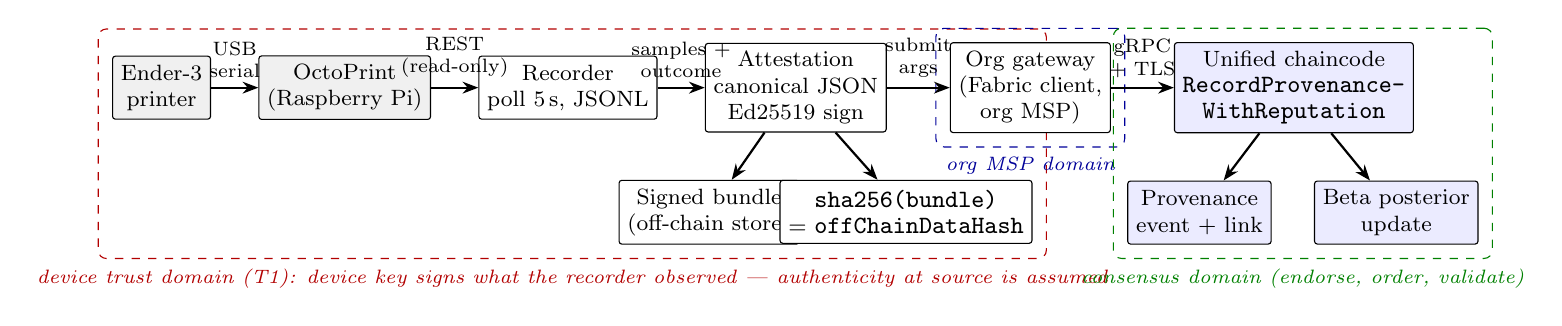
\begin{tikzpicture}[
  font=\footnotesize,
  node distance=4mm and 6mm,
  box/.style={draw, rounded corners=1pt, align=center, inner sep=3pt,
              minimum height=8mm, fill=white},
  hw/.style={box, fill=gray!12},
  chain/.style={box, fill=blue!8},
  arr/.style={-{Stealth[length=2mm]}, thick},
  lbl/.style={font=\scriptsize, midway, align=center},
  boundary/.style={draw, dashed, rounded corners=3pt, inner sep=5pt},
]

% --- Physical / edge nodes ---
\node[hw] (printer) {Ender-3\\printer};
\node[hw, right=of printer] (octo) {OctoPrint\\(Raspberry Pi)};
\node[box, right=of octo] (rec) {Recorder\\poll 5\,s, JSONL};
\node[box, right=of rec] (att) {Attestation\\canonical JSON\\Ed25519 sign};
\node[box, right=8mm of att] (gw) {Org gateway\\(Fabric client,\\org MSP)};
\node[chain, right=8mm of gw] (cc) {Unified chaincode\\\icode{RecordProvenance-}\\\icode{WithReputation}};

% --- Below attestation: the two artifacts it emits ---
\node[box, below=6mm of att, xshift=-11mm] (bundle) {Signed bundle\\(off-chain store)};
\node[box, below=6mm of att, xshift=14mm] (hash) {\icode{sha256(bundle)}\\= \icode{offChainDataHash}};

% --- Below chaincode: ledger effects ---
\node[chain, below=6mm of cc, xshift=-12mm] (event) {Provenance\\event + link};
\node[chain, below=6mm of cc, xshift=13mm] (rep) {Beta posterior\\update};

% --- Edges ---
\draw[arr] (printer) -- node[lbl, above] {USB\\serial} (octo);
\draw[arr] (octo) -- node[lbl, above] {REST\\(read-only)} (rec);
\draw[arr] (rec) -- node[lbl, above] {samples +\\outcome} (att);
\draw[arr] (att) -- node[lbl, above] {submit\\args} (gw);
\draw[arr] (gw) -- node[lbl, above] {gRPC\\+ TLS} (cc);
\draw[arr] (att) -- (bundle);
\draw[arr] (att) -- (hash);
\draw[arr] (cc) -- (event);
\draw[arr] (cc) -- (rep);

% --- Trust boundaries (background layer) ---
\begin{scope}[on background layer]
  \node[boundary, color=red!70!black,
        fit=(printer)(octo)(rec)(att)(bundle)(hash),
        label={[red!70!black, font=\scriptsize\itshape]
               below:device trust domain (T1): device key signs what the
               recorder observed --- authenticity at source is assumed}]
        {};
  \node[boundary, color=blue!60!black, fit=(gw),
        label={[blue!60!black, font=\scriptsize\itshape]below:org MSP
               domain}] {};
  \node[boundary, color=green!50!black, fit=(cc)(event)(rep),
        label={[green!50!black, font=\scriptsize\itshape]below:consensus
               domain (endorse, order, validate)}] {};
\end{scope}

\end{tikzpicture}
}
\caption{The physical-to-chain bridge.  The printer reports temperatures and
job state to OctoPrint; a read-only recorder polls the REST API and appends
samples to a durable log; the attestation module assembles the canonical
bundle, signs it with the device-resident Ed25519 key, and derives the
on-chain commitment as the SHA-256 of the signed bundle
(\icode{offChainDataHash}).  One atomic chaincode invocation records the
provenance event and updates the operator's Beta reputation posterior.
Dashed boxes mark trust domains; the T1 boundary is the device domain.}
\label{fig:pipeline}
\end{figure*}

\subsection{Expected Envelope from the Certified Design}
\label{sec:arch_envelope}

The certified design artifact is the sliced G-code file.  The bridge
derives from it (i) the design identity (SHA-256 over the raw bytes) and
(ii) the \emph{commanded process envelope}: first commanded nozzle and bed
temperatures (\icode{M104}/\icode{M109}, \icode{M140}/\icode{M190}), layer
count, estimated duration, and filament length from the slicer header.
The envelope is what the printer was \emph{told} to do; the telemetry is
what it was \emph{observed} doing.  Binding both into one signed unit lets
any verifier detect divergence later without access to the original file.

\subsection{Canonical Signed Bundle}
\label{sec:arch_bundle}

The bundle (schema \icode{am-provenance/telemetry-bundle/v1};
Listing~\ref{lst:bundle}) contains five blocks: \icode{design} (the
envelope of Section~\ref{sec:arch_envelope}), \icode{observed} (the
telemetry samples, the executed G-code hash, and the actual duration),
\icode{assessment} (Section~\ref{sec:arch_assessment}), \icode{outcome}
(the print server's terminal job event), and the capture \icode{window}.

Serialization is canonical JSON---sorted keys, no insignificant
whitespace, UTF-8---so every verifier, including Go code on a Fabric peer
at the future T2 tier, recomputes byte-identical encodings.  The device
key signs $\mathrm{canon}(\icode{payload})$; the on-chain commitment (the
event's \icode{offChainDataHash}) is
\begin{equation}
h_{\mathrm{oc}} = H\bigl(\mathrm{canon}(\{\icode{payload},
\icode{attestation}\})\bigr),
\label{eq:och}
\end{equation}
where $H$ is SHA-256 and $\mathrm{canon}(\cdot)$ the canonical encoding.
The hash covers the signature itself, so neither block can be swapped
after submission, and verification is two independent checks: recompute
Eq.~\eqref{eq:och} against the ledger value, and verify the signature
over the canonical payload (Section~\ref{sec:eval_tamper}).

\subsection{Observed-versus-Commanded Assessment}
\label{sec:arch_assessment}

The assessment maps physical adherence onto the $[0,1]$ rating dimensions
the reputation engine consumes~\cite{anonymous2026unified}:
\icode{quality} $q$, the fraction of nozzle and bed samples within a
tolerance band ($\pm 8\,^{\circ}$C here) of the commanded envelope;
\icode{compliance} $c$, 1 iff the executed G-code hash equals the
certified design hash, else 0; and \icode{delivery} $d$, 1 if the actual
duration does not exceed the slicer estimate, decaying linearly with
overrun.  The scalar rating submitted with the provenance event is
\begin{equation}
r \;=\; 0.6\,q + 0.25\,c + 0.15\,d .
\label{eq:rating}
\end{equation}
The weights and tolerance band are policy parameters, not claims; we
return to their calibration in Sections~\ref{sec:eval_capture}
and~\ref{sec:discussion}.  Their \emph{relative} ordering, however, is
principled.  \icode{quality} carries the largest weight (0.6) because it is
the only \emph{continuous} physical signal in the vector: it varies
sample-by-sample with the actual process and is therefore the dimension a
fabrication or process-drift attack must move, and the one that degrades
gradually under genuine equipment faults.  \icode{compliance} is weighted
next (0.25) but is \emph{binary and catastrophic}---a mismatch means the
executed design is not the certified one, so its information is mostly
captured by the 0/1 jump rather than by a large coefficient; a high weight
would let many good-quality prints mask a single design substitution, which
is undesirable, while the binary term still vetoes the rating when it
fires.  \icode{delivery} carries the least weight (0.15) because timeliness
is the least security-relevant dimension: a slow print is an operational,
not an integrity, concern, and duration is the easiest quantity for a
cooperative-but-sloppy operator to explain away.  The controlled anomaly of
Section~\ref{sec:eval_anomaly} confirms the ordering empirically---a purely
physical deviation moves \icode{quality} while \icode{compliance} holds.

\subsection{On-Chain Integration}
\label{sec:arch_integration}

The ledger side reuses our unified three-contract
chaincode~\cite{anonymous2026unified} unchanged; the bridge is a new
client of its existing integration path.  One
\icode{IntegrationContract:RecordProvenanceWithReputation} invocation
executes, inside a single Fabric read-write set:

\begin{enumerate}
  \item \textbf{Reputation gate:} if configured for the event type, the
        rated actor's decayed Beta score, event count, and 95\% Wilson
        confidence-interval width are checked before any state is written.
  \item \textbf{Lifecycle transition:} the provenance event (carrying
        \icode{offChainDataHash}) is appended subject to the state machine
        \icode{MATERIAL\_CERTIFIED} $\rightarrow$ \icode{PRINT\_COMPLETE}
        $\rightarrow$ \icode{INSPECTION\_PASSED} $\rightarrow$
        \icode{CERTIFIED}.
  \item \textbf{Stake-gated rating:} the submitter must hold the minimum
        stake (10{,}000 units) and may not rate itself; its rater weight
        $w \in [0.1, 5.0]$ derives from its meta-reputation.
  \item \textbf{Beta update:} for $r \geq 0.5$, $\alpha \mathrel{+}= w
        \cdot r$, else $\beta \mathrel{+}= w \cdot (1-r)$; the score is
        $\alpha/(\alpha+\beta)$ with a Wilson 95\% interval.
  \item \textbf{Bidirectional link:} a
        \icode{PROV\_REP\_LINK} record ties event to rating, and the
        stored event gains a \icode{linkedRatingID}, so audits traverse
        either direction.
\end{enumerate}

Because all five steps share one read-write set, Fabric's commit
semantics make them atomic: no observable state has the physical evidence
on-chain without its reputation consequence, or vice versa.  Prior
measurements put the marginal cost of atomicity at 4.8\,ms (9.9\%) over a
standalone provenance write, with $\sim$337\,B of on-chain metadata per
event~\cite{anonymous2026unified}.

\begin{lstlisting}[float=t, caption={Canonical signed
bundle (abbreviated; real values from the captured run of
Section~\ref{sec:eval_capture}).  The on-chain commitment is the SHA-256
of this object's canonical serialization.}, label={lst:bundle}]
{ "payload": {
    "schema": "am-provenance/telemetry-bundle/v1",
    "assetId": "PART-f4u2-0001",
    "eventType": "PRINT_JOB",
    "machine": "Creality Ender-3",
    "design": {
      "gcode_sha256": "195eabe4...df0986f",
      "slicer": "Cura_SteamEngine 5.12.0",
      "expected_nozzle_c": 200.0,
      "expected_bed_c": 50.0,
      "expected_time_s": 13639, ... },
    "observed": {
      "source": "OCTOPRINT_POLL",
      "tolerance_c": 8.0,
      "actual_time_s": 578,
      "executed_gcode_sha256": "195eabe4...",
      "samples": [ {"t": 1780948249,
        "nozzle_c": 21.45, "bed_c": 21.72,
        "state": "Operational"}, ...115... ] },
    "assessment": { "quality": 0.2,
      "delivery": 1.0, "compliance": 1.0,
      "rating_value": 0.52 },
    "outcome": "PrintCancelled" },
  "attestation": {
    "alg": "Ed25519",
    "device_id": "DEV:1cf20afaacb6ed6b",
    "pubkey": "58363123...2ef0b8c",
    "signature": "15d9a195...b883c0c" } }
\end{lstlisting}

% ===========================================================================
\section{Implementation}
\label{sec:implementation}
% ===========================================================================

All components are implemented and running; nothing in this section is
simulated.

\textbf{Hardware.}  A Creality Ender-3 FDM printer (8-bit Marlin-class
controller, no secure element) driven over USB serial by
OctoPrint~\cite{octoprint} on a Raspberry Pi---a deliberately
representative \emph{legacy} setup, since the installed base of consumer
printers offers no firmware attestation hooks: exactly the fleet T1
targets.

\textbf{Recorder} (\icode{capture\_poll.py}, Python~3).  During a job the
recorder polls OctoPrint's read-only REST endpoints
(\icode{/api/printer}, \icode{/api/job}) every 5\,s, appending each
sample---nozzle and bed actuals and targets, job state---to a durable
JSONL log so a crash loses at most one interval.  When a job it has
observed printing leaves the printing states, it closes the capture and
classifies the outcome (\icode{PrintDone} at $\geq$99.5\% completion, else
\icode{PrintCancelled}).  Polling signs what OctoPrint \emph{reports}; an
event-hook plugin capturing inside the print server is a straightforward
hardening step within the same tier.

\textbf{Attestation module} (\icode{attestation.py}) parses the G-code
envelope, assembles the canonical bundle, and manages the device key.  The
Ed25519 key~\cite{bernstein2012high} is generated on first use and
persists on the bridge host (PKCS\#8 PEM); the device identity
\icode{DEV:}$h_{16}$ is the truncated SHA-256 of the raw public key,
doubling as the T2 registry key.

\textbf{Ledger.}  Hyperledger Fabric v3.1.0 (two organizations, Raft
ordering, TLS) running the unified chaincode
of~\cite{anonymous2026unified} as Chaincode-as-a-Service.  The submission
script drives the lifecycle:
\icode{CreateMaterialCertification} binds the asset to the certified
design hash, then \icode{RecordProvenanceWithReputation} commits the
print-job event with the bundle hash, the derived rating
(Eq.~\eqref{eq:rating}), and the payload's evidence hash; six queries
(asset, history, linked ratings, reputation, trust report) verify the
committed state end-to-end.

The bridge required no chaincode changes: the existing
\icode{offChainDataHash} field and integration path absorb the
attestation layer as designed---evidence that hash-anchored provenance
schemas generalize to authenticated evidence without ledger migration.

% ===========================================================================
\section{Evaluation}
\label{sec:evaluation}
% ===========================================================================

The evaluation answers four questions: (Q1)~does the pipeline produce a
verifiable, on-chain-anchored evidence record from a real print job;
(Q2)~does physical adherence propagate into a meaningful reputation
update; (Q3)~is tampering with stored evidence detected; (Q4)~what are
the bridge's latency and storage costs.  All four are answered with
measured data from \textbf{five real print jobs} on the Ender-3 testbed,
spanning \textbf{three geometries} (a complex 5\,MB part, a calibration
cube, and a functional mounting bracket) and \textbf{three outcome types}
(completed, cancelled, and a deliberately injected thermal anomaly).
Table~\ref{tab:runs} summarizes the runs; the subsections that follow
walk through a detailed case study, the controlled anomaly comparison,
reputation propagation, tamper detection, and the cost measurements.

\begin{table*}[t]
\centering
\caption{The five real print jobs: three geometries, three outcome types.
All bundles verify (Ed25519 signature and ledger-hash check) and all carry
\icode{compliance}~$=1.0$ (executed G-code hash equals the certified
design).  \icode{q}/\icode{c}/\icode{d} are the assessment dimensions of
Eq.~\eqref{eq:rating}; canonical size is the off-chain signed bundle, whose
on-chain footprint is a constant 369\,B regardless of bundle size.}
\label{tab:runs}
\small
\begin{tabular}{lllccccrrr}
\toprule
Run & Geometry & Outcome & \icode{q} & \icode{c} & \icode{d} & rating $r$
  & samples & canon.\ B & on-chain B \\
\midrule
\icode{f4u2}        & complex (5.0\,MB) & PrintCancelled & 0.200 & 1.0 & 1.000 & 0.520 & 115 & 13{,}408 & 369 \\
\icode{cube\_done}  & calibration cube  & PrintDone      & 0.780 & 1.0 & 0.105 & 0.734 & 115 & 13{,}528 & 369 \\
\icode{cube\_anomaly}& calib.\ cube (+15\,$^{\circ}$C) & PrintDone & 0.708 & 1.0 & 0.271 & 0.715 & 105 & 12{,}459 & 369 \\
\icode{cube\_repeat}& calibration cube  & PrintDone      & 0.936 & 1.0 & 1.000 & 0.962 & 56  & 7{,}214  & 369 \\
\icode{bracket}     & L-bracket (functional) & PrintDone & 0.847 & 1.0 & 1.000 & 0.908 & 84  & 10{,}213 & 369 \\
\bottomrule
\end{tabular}
\end{table*}

%                         --
\subsection{Live Capture Case Study (Q1)}
\label{sec:eval_capture}
%                         --

We first walk through one run end-to-end.  A print job for asset
\icode{PART-f4u2-0001} was executed on the Ender-3 from \icode{f4u2.gcode}
(4{,}998{,}971\,B, SHA-256 \icode{195eabe4\ldots}, sliced with Cura 5.12.0:
55 layers, estimated 13{,}639\,s, commanded envelope 200\,$^{\circ}$C
nozzle / 50\,$^{\circ}$C bed).  The recorder captured \textbf{115 samples}
at a $\sim$5\,s interval over a 578\,s window; the operator cancelled the
job shortly after both heaters reached their setpoints---a deliberately
imperfect run, chosen here as the \icode{PrintCancelled} exemplar and more
informative for the rating pipeline than a flawless one.

Marlin heats sequentially: the log records \icode{Operational}
$\rightarrow$ \icode{Printing}, the bed ramps 21.8 $\rightarrow$
50\,$^{\circ}$C in ${\approx}90$\,s, then the nozzle 21.9 $\rightarrow$
200\,$^{\circ}$C in a further ${\approx}96$\,s.  At cancellation both
targets drop to zero and the state returns to \icode{Operational},
correctly classified as \icode{PrintCancelled}.

\textbf{Assessment.}  Applying the policy of
Section~\ref{sec:arch_assessment}: \icode{compliance} $= 1.0$ (executed
G-code hash matches the certified design), \icode{delivery} $= 1.0$
(578\,s $\leq$ 13{,}639\,s estimate), and \icode{quality} $= 0.2$
(46 of 230 nozzle+bed readings within $\pm 8\,^{\circ}$C of target),
yielding $r = 0.6(0.2) + 0.25(1.0) + 0.15(1.0) = \mathbf{0.52}$.  The low
quality score is dominated by the idle and heat-up samples preceding the
setpoints, which the current policy counts against the target---a
conservative artifact we flag for calibration
(Section~\ref{sec:discussion}) rather than tune away post hoc.

\textbf{Commitment.}  The signed bundle canonicalizes to 13{,}408\,B; its
commitment, stored in the \icode{PRINT\_JOB} event's
\icode{offChainDataHash} field, is
\icode{9b739c985110272a79d847b2f5507ea6}\allowbreak
\icode{29b2358e3519fc06af47f7783459d812}.  The on-chain footprint remains
the $\sim$337\,B structured record of~\cite{anonymous2026unified}; the
36$\times$ larger evidence bundle stays off-chain under device signature
\icode{DEV:1cf20afaacb6ed6b}.  All five runs reproduce this Q1 property:
each produced a bundle that verifies by both the recomputed ledger hash
and the Ed25519 signature (Table~\ref{tab:runs}).

%                         --
\subsection{Controlled Thermal-Anomaly Comparison}
\label{sec:eval_anomaly}
%                         --

The headline result is a controlled A/B between two physically identical
prints of the calibration cube, captured from the same idle start so that
heat-up samples enter both assessments equally.  In \icode{cube\_anomaly},
a mid-print setpoint override (\icode{M104 S215}, $+15\,^{\circ}$C) was
injected via the OctoPrint terminal once the nozzle had stabilized at
200\,$^{\circ}$C, held for 60\,s, then reverted to 200\,$^{\circ}$C.
Figure~\ref{fig:thermal} shows the captured excursion: the nozzle climbs
to 215\,$^{\circ}$C, holds, and recovers---14 samples leave the
$\pm 8\,^{\circ}$C tolerance band.

The effect on the rating is exactly the intended one.  Relative to the
normal print (\icode{cube\_done}, \icode{quality}~$=0.780$, 103/132
in-tolerance), the anomaly run scores \icode{quality}~$=0.708$ (92/130
in-tolerance): a \textbf{9.3\% relative drop in quality} attributable
solely to the injected deviation.  Crucially, \icode{compliance} stays
$1.0$ across both runs---the certified \emph{design} was never
altered---so the bridge attributes the degradation to physical execution,
not to a design substitution.  This separation of ``what was supposed to
be made'' (compliance) from ``how faithfully it was made'' (quality) is
the property a provenance consumer needs, and it is recovered here from
telemetry alone on unmodified consumer hardware.

We treat \icode{cube\_done} versus \icode{cube\_anomaly} as the clean
comparison because both share an idle-start capture.  The third normal
print, \icode{cube\_repeat}, scores higher (\icode{quality}~$=0.936$) only
because its recorder attached after warm-up ($\sim$2.6\% progress), so the
out-of-tolerance heat-up samples are absent; we report it as an additional
completed-print data point but not as a controlled comparison, to avoid
overclaiming (Section~\ref{sec:discussion}).

\begin{figure}[t]
\centering
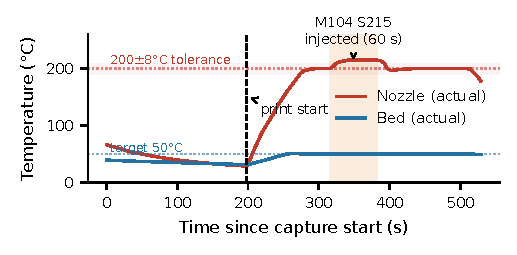
\includegraphics[width=\columnwidth]{fig_thermal_trace}
\caption{Real thermal telemetry from the \icode{cube\_anomaly} run (105
OctoPrint samples, 5\,s interval).  The dashed vertical marks the logged
print-start transition; the shaded orange band marks the 60\,s window in
which \icode{M104 S215} was injected, driving the nozzle (red) out of the
$\pm 8\,^{\circ}$C tolerance band (shaded red) before recovery.  The bed
(blue) holds 50\,$^{\circ}$C throughout.}
\label{fig:thermal}
\end{figure}

%                         --
\subsection{Reputation Propagation (Q2)}
\label{sec:eval_reputation}
%                         --

Each run's rating was submitted on the \icode{quality} dimension against
operator \icode{operator-secnet} via the atomic
\icode{RecordProvenanceWithReputation} invocation.  Starting from the
prior $\mathrm{Beta}(2.0, 2.0)$, the first (f4u2) submission of $r=0.52$
with rater weight $w=0.657$ moved the posterior to
$\mathrm{Beta}(2.34, 2.0)$, i.e.\ score $0.539$ with 95\% Wilson interval
$[0.179, 0.863]$.  Because every subsequent rating exceeded $0.5$, the
$\beta$ pseudocount stayed at $2.0$ and the score rose monotonically as
evidence accumulated.  After all five committed events
(\icode{totalEvents}~$=5$) the on-chain posterior is
$\mathrm{Beta}(4.95, 2.0)$: \textbf{score $0.712$}, 95\% Wilson interval
$[0.356, 0.917]$.

Figure~\ref{fig:beta} plots this measured trajectory.  Two properties
matter.  First, no single print dominates: one mediocre run neither
condemns nor absolves the operator, the intended Bayesian behavior.
Second, the interval tightens as evidence accumulates---its width shrinks
from \textbf{0.684 at $n{=}1$ to 0.561 at $n{=}5$}---so the
confidence-interval gate becomes progressively easier to clear with
attested history and \emph{absence} of history has consequences, closing
the selective-reporting loophole of Section~\ref{sec:boundary}.  Five jobs
is still early in the curve; the trend, not the absolute width, is the
result.

\begin{figure}[t]
\centering
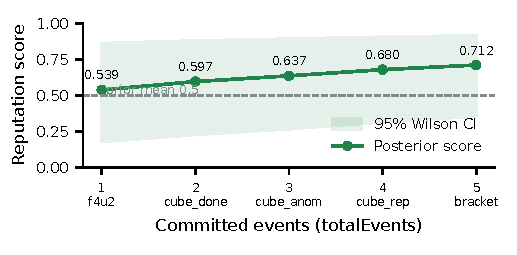
\includegraphics[width=\columnwidth]{fig_beta_posterior}
\caption{Measured on-chain reputation evolution for \icode{operator-secnet}
(quality dimension) across the five committed events.  The score rises
$0.539 \rightarrow 0.712$ and the 95\% Wilson interval (shaded) tightens
from width $0.684$ to $0.561$ as attested evidence accumulates.  Values are
read directly from the ledger after each submission.}
\label{fig:beta}
\end{figure}

%                         --
\subsection{Tamper Detection (Q3)}
\label{sec:eval_tamper}
%                         --

To exercise the post-hoc-tampering row of Table~\ref{tab:taxonomy}, a
single observed nozzle sample in a stored bundle was altered to
235\,$^{\circ}$C.  Verification against the ledger then fails twice,
independently: the recomputed bundle hash no longer matches the on-chain
\icode{offChainDataHash} (Eq.~\eqref{eq:och}), and the Ed25519 signature
over the canonical payload is invalid.  The redundancy matters: detection
survives either a compromised ledger view (signature still fails) or a
leaked device key used to re-sign altered evidence (the ledger hash still
mismatches, because the commitment covers the original signature).  Only
an adversary who can both re-sign \emph{and} rewrite committed Fabric
state---defeat the endorsement policy---evades both checks.

%                         --
\subsection{Latency and Storage Cost (Q4)}
\label{sec:eval_cost}
%                         --

\textbf{Bridge latency (Q4a).}  We instrumented each pipeline stage and
timed it over 100 iterations on each of the four PLA-profile runs
(cube\,$\times$3, bracket).  Figure~\ref{fig:cost}a reports the per-stage
mean with a P95 cap.  The full attest pipeline---parse, payload assembly,
canonicalization, Ed25519 signing, and hash derivation---completes in a
\textbf{0.91\,ms mean}; adding independent verification (signature plus
hash recompute) brings the round trip to \textbf{1.55\,ms}.  Signing
(0.32\,ms) and verification (0.63\,ms) dominate, as expected for Ed25519
over a $\sim$13\,kB payload.  This bridge-side cost is negligible beside
the ledger commit: prior chaincode-side measurement put the atomic
provenance+reputation write at 53.6\,ms mean on the same-host
testbed~\cite{anonymous2026unified}, so the attestation layer adds under
3\% to end-to-end latency.  G-code parsing is the one size-dependent stage:
0.08\,ms for the $\sim$20--38\,kB cube/bracket files but 11.4\,ms for the
5\,MB \icode{f4u2.gcode}---parse scales with design size while signing does
not, because signing covers the fixed-size hash, not the raw G-code.

\textbf{Bundle-size scaling (Q4b).}  Canonical bundle size grows with the
number of retained telemetry samples---from 7.2\,kB (56 samples) to
13.5\,kB (115 samples) across the five runs (Figure~\ref{fig:cost}b)---but
the \textbf{on-chain footprint is a constant 369\,B} (a 32-byte evidence
hash plus the $\sim$337\,B structured record), independent of bundle size.
Compression of the off-chain bundle to its on-chain commitment ranges
19.5$\times$--36.7$\times$.  Linear extrapolation of the per-sample growth
suggests multi-hour prints at 5\,s sampling reach low-single-digit MB
off-chain while the ledger cost stays fixed, motivating the
windowed-summary policies discussed in Section~\ref{sec:discussion}; the
on-chain side already scales independently of print duration.

\begin{figure}[t]
\centering
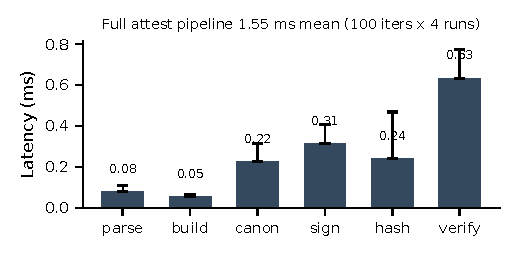
\includegraphics[width=0.49\columnwidth]{fig_bridge_latency}\hfill
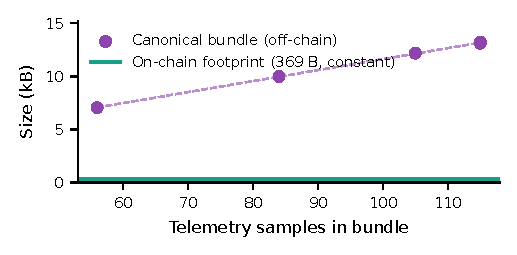
\includegraphics[width=0.49\columnwidth]{fig_bundle_scaling}
\caption{Measured costs.  (a)~Per-stage bridge latency (mean bar, cap at
P95), averaged over 100 iterations on each of the four PLA-profile runs;
the full pipeline incl.\ verification is 1.55\,ms.  (b)~Canonical
off-chain bundle size versus retained samples (five runs); the on-chain
footprint (green) is constant at 369\,B.}
\label{fig:cost}
\end{figure}

% ===========================================================================
\section{Discussion}
\label{sec:discussion}
% ===========================================================================

\subsection{What T1 Buys, and What It Honestly Does Not}

The captured run demonstrates the T1 claim precisely: after the device
signs, every byte of evidence is bound to the ledger, and single-sample
tampering is detected by two independent mechanisms.  It equally
demonstrates the boundary: had the bridge host synthesized the entire
115-sample trace before signing, nothing downstream could tell.  We regard
stating this boundary as a contribution in itself.  A certifying authority
needs to know that a T1 record means ``this evidence has not changed since
the device signed it,'' not ``this print happened as described.''  For the
dominant practical threats---retroactive editing when a part later fails,
reuse of good evidence, quiet design substitution---tamper-evidence after
signing is exactly the needed property, deployable today on unmodified
consumer hardware.

\subsection{Path to T2 and T3}

T2 requires no new cryptography: the device identity and raw public key
already exist in the bundle, and the chaincode gains a registry keyed by
device ID with enrollment, revocation, and endorsement-time Ed25519
verification of the bundle.  Its value is organizational: enrollment
becomes a ledger event subject to endorsement policy, so a stolen key is
bounded by its revocation window and a bureau cannot quietly add signing
devices.  T3 addresses fabrication at source---key in a TEE or secure
element, measured boot of the recorder, and, on industrial machines,
signing at the sensor or controller level.  Threshold attestation across
independent observers (e.g., a bureau device plus a customer-supplied
witness camera or power monitor) raises collusion cost without trusted
hardware on the printer.  Even T3, honestly, does not defeat
physical-world spoofing (a detached thermistor in a heated block):
attestation raises the cost and forensic visibility of fraud; it does not
make physics self-authenticating.

\subsection{Assessment-Policy Calibration}

The quality score of 0.2 for the cancelled run, whose steady-state
tracking was tight ($\pm 0.5\,^{\circ}$C at setpoint), shows the current
policy is miscalibrated for short runs: idle and ramp samples, during which
targets are legitimately unmet, dominate the in-tolerance fraction.  The
five-run data makes the effect precise: the two idle-started cubes score
0.78--0.71 despite excellent steady-state tracking, whereas
\icode{cube\_repeat}, captured after warm-up, scores 0.94---the
$\approx$0.16 spread is almost entirely the heat-up artifact, not a
difference in print fidelity.  The fix is phase-aware scoring (weighting
only printing-phase samples), but we report the uncalibrated numbers
because the methodological point stands regardless: the policy is
transparent and deterministic, encoded in the signed bundle itself, so any
party can recompute and contest a rating from the evidence---unlike
subjective ratings, which are unfalsifiable.

\subsection{Limitations}

(i)~The recorder polls OctoPrint's REST API rather than hooking its event
bus, adding one software layer inside the T1 trust domain.  (ii)~A 5\,s
poll can miss sub-interval transients; the thermal-anomaly run of
Section~\ref{sec:eval_anomaly} captured a 60\,s excursion comfortably, but
faster transients would require event-bus hooking or a shorter interval.
(iii)~The evaluation is single-printer, five-job, three-geometry: the
remaining gap is breadth across \emph{machines and sites}, not across jobs
or part shapes.  One of the five runs (\icode{cube\_repeat}) had its
recorder attach after warm-up, so we use it only as a completed-print data
point and reserve the controlled quality comparison for the two
idle-started cube runs---a reminder that capture must begin before heating
for heat-up samples to be scored consistently.  (iv)~Outcome
classification cannot separate cancellation from failure; the event-hook
plugin can.  (v)~Bundle growth is linear in duration; summarization
policies that retain raw extremes while downsampling steady state are
future work.  (vi)~A read-only ledger query
(\icode{GetAssetHistory}) currently fails an output-schema check
(\icode{linkedRatingID}) on history events; this is a query-path defect
only---all write-path commitments and the reputation updates of
Section~\ref{sec:eval_reputation} succeed and verify---but it should be
fixed before the trust-report view is relied upon operationally.

% ===========================================================================
\section{Conclusion}
\label{sec:conclusion}
% ===========================================================================

On-chain provenance for additive manufacturing is only as trustworthy as
the bridge that carries physical evidence onto the ledger.  This paper
made that bridge the object of study: a four-tier trust analysis with
explicitly stated boundaries; a canonical, device-signed bundle binding
certified design, commanded envelope, observed telemetry, and outcome
into one Ed25519-signed unit anchored by a single on-chain hash; and a
working T1 implementation on unmodified consumer hardware integrated with
a Fabric v3.1.0 provenance--reputation chaincode.  Across five real print
jobs spanning three geometries and three outcome types, each run became a
7--14-kB signed bundle anchored by a constant 369-B on-chain footprint and
an atomic update of the operator's Beta posterior; a controlled
$+15\,^{\circ}$C injection lowered the derived quality score by 9.3\% while
design-hash compliance held at 1.0, and a single flipped sample was caught
by both the ledger-hash and device-signature checks.  The attestation
pipeline costs 1.55\,ms, under 3\% of the ledger-commit time.  The honest
residual---T1 cannot detect fabrication at source by the device-key
holder---defines the agenda: the T2 on-chain device registry, T3
hardware-rooted or threshold attestation, and evaluation across multiple
machines and sites.


% \section*{Acknowledgment}
% ...

\balance
\bibliographystyle{IEEEtran}
\bibliography{references}

\end{document}
